\chapter{Dispositif expérimental}

%\section{Les accélérateurs de particules}

La particule élémentaire la plus massive du Modèle Standard est le quark top, avec une masse d'environ \SI{173}{\GeV}. Afin d'explorer des zones où peuvent se situer de la nouvelle physique, il est nécessaire de fournir des énergies bien supérieures à cette masse. On utilise pour cela des accélérateurs de particules, qui permettent de faire collisionner deux particules accélérées à grande énergie, afin de produire d'autres particules plus massives. On distingue deux grands types d'accélérateurs : les accélérateurs linéaires et les accélérateurs circulaires.
\begin{itemize}
  \item Les accélérateurs linéaires sont les moins puissants. En effet, les particules sont accélérées à l'aide d'un champ électrique le long d'une ligne droite. L'énergie est donc directement proportionnel à la longueur.
  \item Les accélérateurs circulaires peuvent atteindre des énergies très importantes. Les particules sont accélérées dans des cavités circulaires, ce qui permet d'augmenter l'énergie à chaque tour. 
\end{itemize}

\section{Le Large Hadron Collider (LHC)}

Le grand collisionneur de hadrons est à ce jour le plus grand et le plus puissant accélérateur de particules au monde. Il est installé en lieu et place du LEP (\emph{Large Electron Positron collider}), dans un tunnel de \SI{27}{\km} de circonférence, enfoui à plus de \SI{100}{\m} au dessous de la surface. Géographiquement, le LHC est situé à la frontière Franco-Suisse, sur le site du CERN (Organisation Européenne pour la Recherche).

Composé de deux anneaux, le LHC permet d'accélérer des protons a des énergies de \SI{7}{\TeV}, grâce à environ 9500 aimants. Une fois refroidit à une température de \SI{1.8}{\K} grâce à de l'hélium super fluide, ces aimants deviennent supraconducteur et délivre un champ magnétique nominal de \SI{8.33}{\tesla}, champ qui permet de courber les protons afin de leur garantir une trajectoire circulaire.

Le premier faisceau a circulé au LHC le 10 septembre 2008. Malheureusement, le 19 septembre 2008, un incident de cryogénie entraînât une interruption de plus d'un an, et ce n'est que le 20 novembre 2009 que les anneaux du LHC accueillir de nouveau des protons. A partir du 23 novembre, les premières collisions $pp$ destinées à la physique ont commencés à être enregistrer par les détecteurs. S'en suivirent 3 années de montée en puissant progressive, passant d'une énergie de \SI{7}{\TeV} dans le centre de masse en 2010-2011 à \SI{8}{\TeV} en 2012. Au moment de la rédaction de ce manuscrit, le LHC est arrêté pour environ 2 ans. Cet arrêt planifié est mis à profit principalement afin de mettre à jours les détecteurs. Les collisions $pp$ pour la physique devrait reprendre en septembre 2015.

\subsection{L'accélération des protons}
Avant d'atteindre leur énergie nominale dans l'anneau du LHC, les protons sont accélérés graduellement le long de différents accélérateurs :

\begin{figure} \centering
  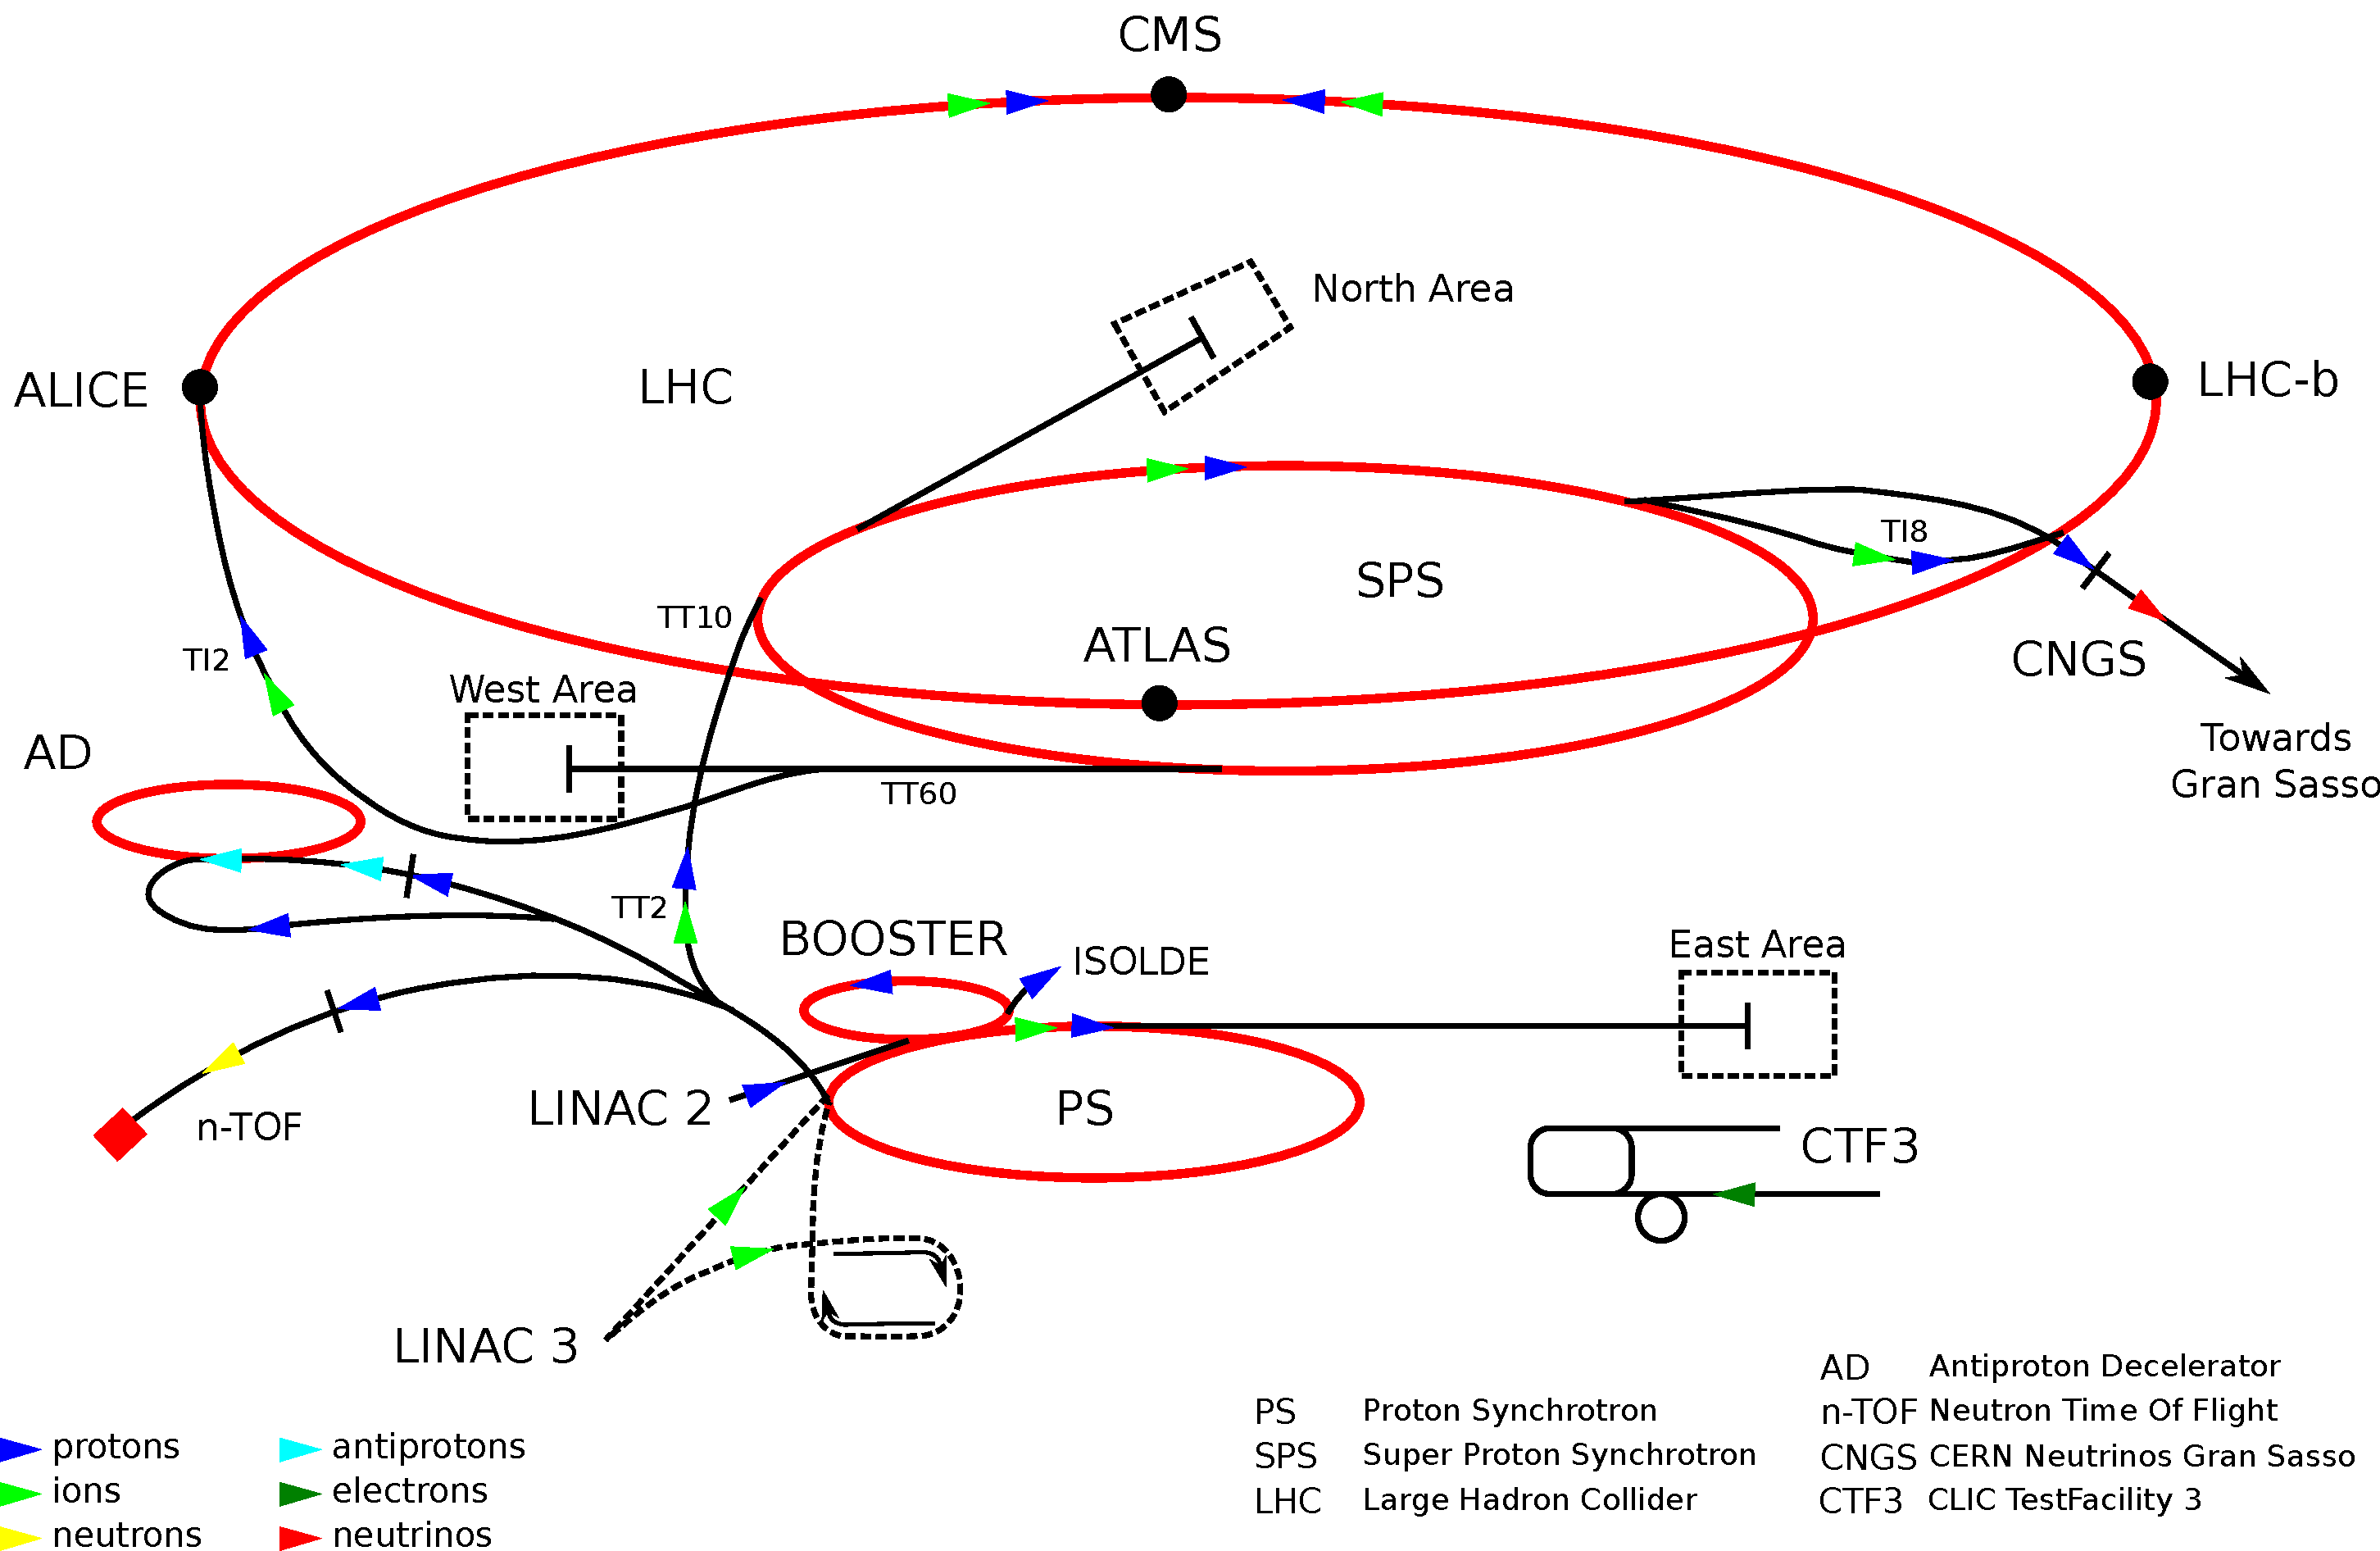
\includegraphics[width=0.7\textwidth]{Cern-accelerator-complex.pdf}
  \caption{Le complexe d'accélérateurs du CERN}
  \label{fig:lhc_complex}
\end{figure}

\begin{description}
  \item[Le LINAC 2 (1978)] Tout commence par une simple bouteille d'hydrogène. Un champ électrique ionise le gaz afin d'arracher les électrons du noyau. Les protons restant sont accélérés jusqu'à une énergie de \SI{50}{\MeV}.
  \item[Le \emph{Proton Synchroton Booster} (PSB -- 1972)] Le faisceau est ensuite injecté dans le PSB, un accélérateur circulaire, où les protons atteignent une énergie de \SI{1.4}{\GeV}.
  \item[Le \emph{Proton Synchroton} (PS -- 1959)] Dans cet accélérateur, les protons atteignent une énergie de \SI{25}{GeV}.
  \item[Le \emph{Super Proton Synchroton} (SPS -- 1976)] Le faisceau subit sa dernière étape d'accélération dans le SPS, atteignant cette fois ci une énergie de \SI{450}{\GeV}, avant d'être injecté dans le LHC et accéléré pour atteindre l'énergie nominale de \SI{7}{\TeV} par faisceau.
  %\item[Le LHC] L'énergie du faisceau est suffisante pour atteindre l'anneau du LHC. Il est cette fois accéléré jusqu'à l'énergie nominale.
\end{description}

Un schéma descriptif de la chaîne d'accélération du CERN est présenté figure \ref{fig:lhc_complex}

\subsection{La luminosité}

La luminosité instantanée est une variable clé d'un accélérateur de particule. Exprimée en \si{\per\square\cm\per\second}, elle caractérise le nombre de collision par seconde et par centimètre carré. On l'exprime au LHC en fonction de diverses variables caractéristique de la forme des paquets de protons,
de l'énergie, de la séparation des paquets, \ldots~On a
\begin{align*}
  \mathcal{L}_{\text{inst}} &= \frac{\gamma\,f\,n_p\,N_p^2}{4\pi\,\epsilon_n\,\beta_*} = \frac{f\,n_p\,N_p^2}{4\pi\,\sigma_x\,\sigma_y}
\end{align*}
où $\gamma$ est le boost de Lorentz, $f$ la fréquence de révolution des paquets, $n_p$ le nombre de paquets de protons, $N_p$ le nombre de protons par paquets, $\epsilon_n$ l'émittance transverse\footnote{L'émittance est une mesure de la parallélité du faisceau}, $\beta^*$ la fonction d'amplitude\footnote{$\beta^*$ est la distance entre le point d'interaction et l'endroit où le faisceau double de largeur} et $\sigma_x,y$ les tailles transverses du faisceau au point d'interaction. La valeur des différents paramètres du faisceau est donné table \ref{tab:lhc_beam} pour les trois années de fonctionnement.

\begin{figure} \centering
  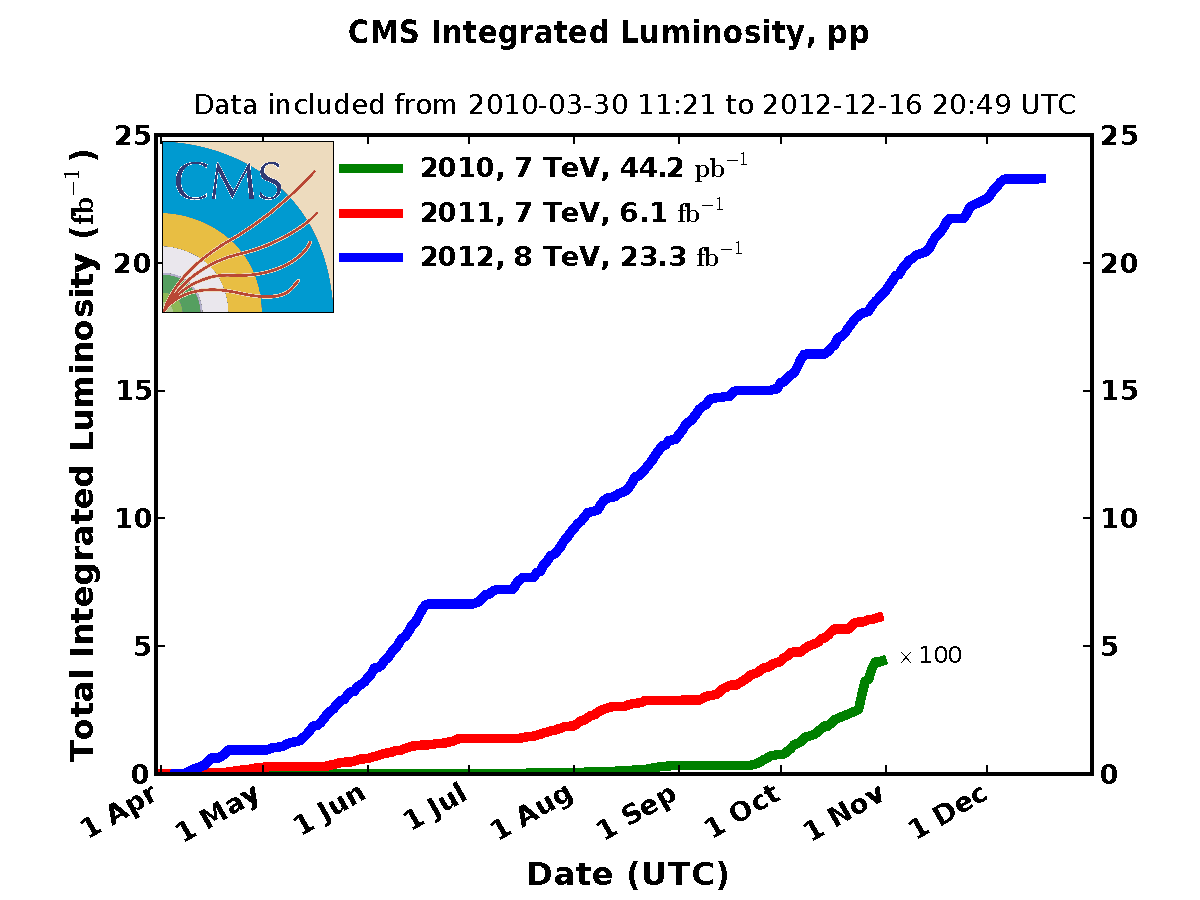
\includegraphics[width=0.7\textwidth]{chapitre2/figs/CMS_lumi.pdf}
  \caption{Luminosité intégrée collectée par l'expérience CMS au cours des années 2010 (vert), 2011 (rouge) et 2012 (bleu). La distribution de la luminosité collectée a été zoomé 100x pour pouvoir la distingué sur le graphique.}
  \label{fig:lumi}
\end{figure}

\begin{table} \centering
  \begin{tabular}{@{}ccccc@{}} \toprule
  \multirow{2}{*}{Caractéristiques} & \multicolumn{4}{c}{Conditions} \\ \cmidrule{2-5}
  & nominales & 2010 & 2011 & 2012 \\ \midrule
  Énergie par faisceau (\si{\TeV}) & 7 & \num{3.5} & \num{3.5} & \num{4} \\
  $\mathcal{L}_\text{inst}$ (\si{\per\square\cm\per\s}) & \num{e34} & \num{2.1e32} & \num{3.7e33} & \num{7.7e33}\\
  $\mathcal{L}$ (\si{\invfb}) & 100 & \num{36e-3} & \num{4.98} & \num{19.7} \\ \midrule
  Temps entre paquet (\si{\ns}) & 25 & > 150 & 75 / 50 & 50 \\
  Nombre de paquets & 2808 & 368 & 1092 & 1380\\
  Protons par paquets (\num{e11}) & \num{1.15} & \num{1.2} & \num{1.45} & \num{1.7}\\
  $\beta^*$ (\si{\m}) & \num{0.55} & \num{2.0} - \num{3.5} & \num{1.0} - \num{1.5} & \num{0.6} \\ \bottomrule
  \end{tabular}
  \caption{Les différents paramètres du faisceau $pp$ du LHC pour les trois premières années de fonctionnement}
  \label{tab:lhc_beam}
\end{table}

\medskip

On obtient la luminosité totale en intégrant $\mathcal{L}_{\text{inst}}$ sur la durée de prise de donnée, $\mathcal{L} = \int \mathcal{L}_\text{inst} dt$. C'est grâce à cette luminosité que l'on quantifie la quantité de données disponible (statistique) pour les expériences. En effet, le nombre d'événements produit par les collisions pour un processus donné est
\begin{align*}
  N &= \mathcal{L} \sigma
\end{align*}
où $\sigma$ est la section efficace du processus. On voit donc que pour une section efficace donnée, le nombre d'événements produit est directement proportionnel à la luminosité. Il est donc primordiale d'avoir une luminosité instantanée la plus grande possible et une durée de prise de données la plus longue possible afin d'être en mesure d'observer des processus rare. On peut voir figure \ref{fig:lumi} la distribution de la luminosité collectée par l'expérience CMS (section \ref{sec:cms}) au cours de 3 années de prise de données.

\bigskip

Bien qu'opérant actuellement à des énergies presque deux fois plus faible que celles prévues par les conditions nominales, le LHC est déjà capable de fournir une luminosité instantanée pic équivalente à celle sensée être obtenue à \SI{14}{\TeV}. Cela laisse présager d'excellentes performances lors de la reprise en 2015.

\subsection{L'empilement}

Lors d'un croisement de paquets de protons, plusieurs interactions $pp$ peuvent avoir lieu : la collision principale forme l'événement dur, et c'est celle ci qu'on souhaite étudier. Les autres collisions (élastiques ou inélastiques) viennent parasiter la collision principale, et se superposent à l'événement dur. Cet effet est communément appelé empilement (pileup (PU) en anglais). Le nombre d'événement de PU par collision dépend de la configuration du LHC. En 2012, on l'estime à environ 15, et il prévu qu'il passe a environ 25 lors de la reprise en 2015.

\medskip

On distingue deux types d'empilement différent : celui produit en même temps que l'événement dur est le plus handicapant, puisqu'il va entraîner de l'activité non désirés au sein du détecteur, et ainsi perturber la reconstruction des particules produites lors de la collision principale. C'est le PU "in-time". On distingue aussi le PU "out-of-time", causé par des particules produites lors des croisements de paquets antérieurs ou postérieurs. Ces particules peuvent mettre du temps à se désintégrer ou à être détecté, et elles viennent donc interférer avec la mesure de la collision principale.

\subsection{Les expériences}

Le LHC étant un collisionneur circulaire, il est possible de faire se croiser les faisceaux de protons à plusieurs endroits. On peut donc installer plusieurs dispositifs expérimentaux, un à chaque point de croisement. Le LHC compte 4 points de croisements, et donc 4 expériences majeures : ALICE \citep{alice}, ATLAS \citep{atlas}, CMS \citep{cms} et LHCb \citep{lhcb}.

\begin{description}
  \item[A Large Ion Collider Experiment (ALICE)] Cette expérience est principalement dédiée à l'étude du déconfinement de la matière nucléaire, le plasma de quark et gluon. Les données qu'elle utilise sont celles issues des collisions d'ions lourds ($pB-pB$), mais les collisions $pp$ sont aussi utilisées afin de calibrer le détecteur.
  \item[A Toroidal LHC ApparatuS (ATLAS) / Compact Muon Solenoid (CMS)] Ce sont les deux expériences généralistes du LHC. En effet, le programme de physique de ATLAS et CMS est très vaste, et couvre la recherche du boson de Higgs et de nouvelles physiques, les mesures de précisions du Modèle Standard, ainsi que la recherche de candidate matière noire. Souvent mises en concurrence, ces expériences sont pourtant complémentaires. Ainsi, on a pu voir le 4 juillet 2012 ces deux expériences annoncer conjointement la découverte d'une particule compatible avec le boson de Higgs \citep{higgs_atlas,higgs_cms}, chacune confirmant ainsi les résultats de l'autre.
  \item[Large Hadron Collider beauty (LHCb)] C'est la dernière expérience majeure du LHC, et est principalement dédiée à la mesure de précision du Modèle Standard ainsi qu'a l'étude de la violation de la symétrie CP, grâce à l'étude poussée du quark $b$. La collaboration LHCb a d'ailleurs annoncé récemment avoir observé pour la première fois la violation de symétrie CP dans le système $B_s$ \citep{lhcb_bs}, tel que prévu par le Modèle Standard. Cette récente découverte permet de contraindre encore plus fortement certains modèle de nouvelles physiques.
\end{description}

En plus de ces 4 expériences majeures, on trouve 3 autres expériences au LHC, installées à proximité des points de croisement des faisceaux : LHCf \citep{lhcf}, MoEDAL \citep{moedal} et TOTEM \citep{totem}.

\begin{description}
  \item[Large Hadron Collider forward] Située a environ \SI{140}{\m} de part et d'autre de ATLAS, ce détecteur étudie les particules créées à très petits angles, principalement afin de simuler la production de rayon cosmiques de très haute intensité en laboratoire.
  \item[Monopole and Exotics Detector at the LHC (MoEDAL)] Située juste en aval de LHCb, MOeDAL traque les monopôles magnétiques, grâce a un détecteur spécialement conçu pour ce rôle.
  \item[TOTal Elastic and diffractive cross section Measurement (TOTEM)] Destinée à la mesure précise de la luminosité du LHC, cette expérience étudie les particules créées à très petits angles. Elle peut ainsi mesurer la section efficace élastique des collisions $pp$.
\end{description}

% \bigskip
% 
% Les travaux effectués dans cette thèse ont tous été réalisés à l'aide des données prise par le détecteur CMS. Voyons

\section{L'expérience Compact Muon Solenoid (CMS)} \label{sec:cms}

\begin{figure} \centering
  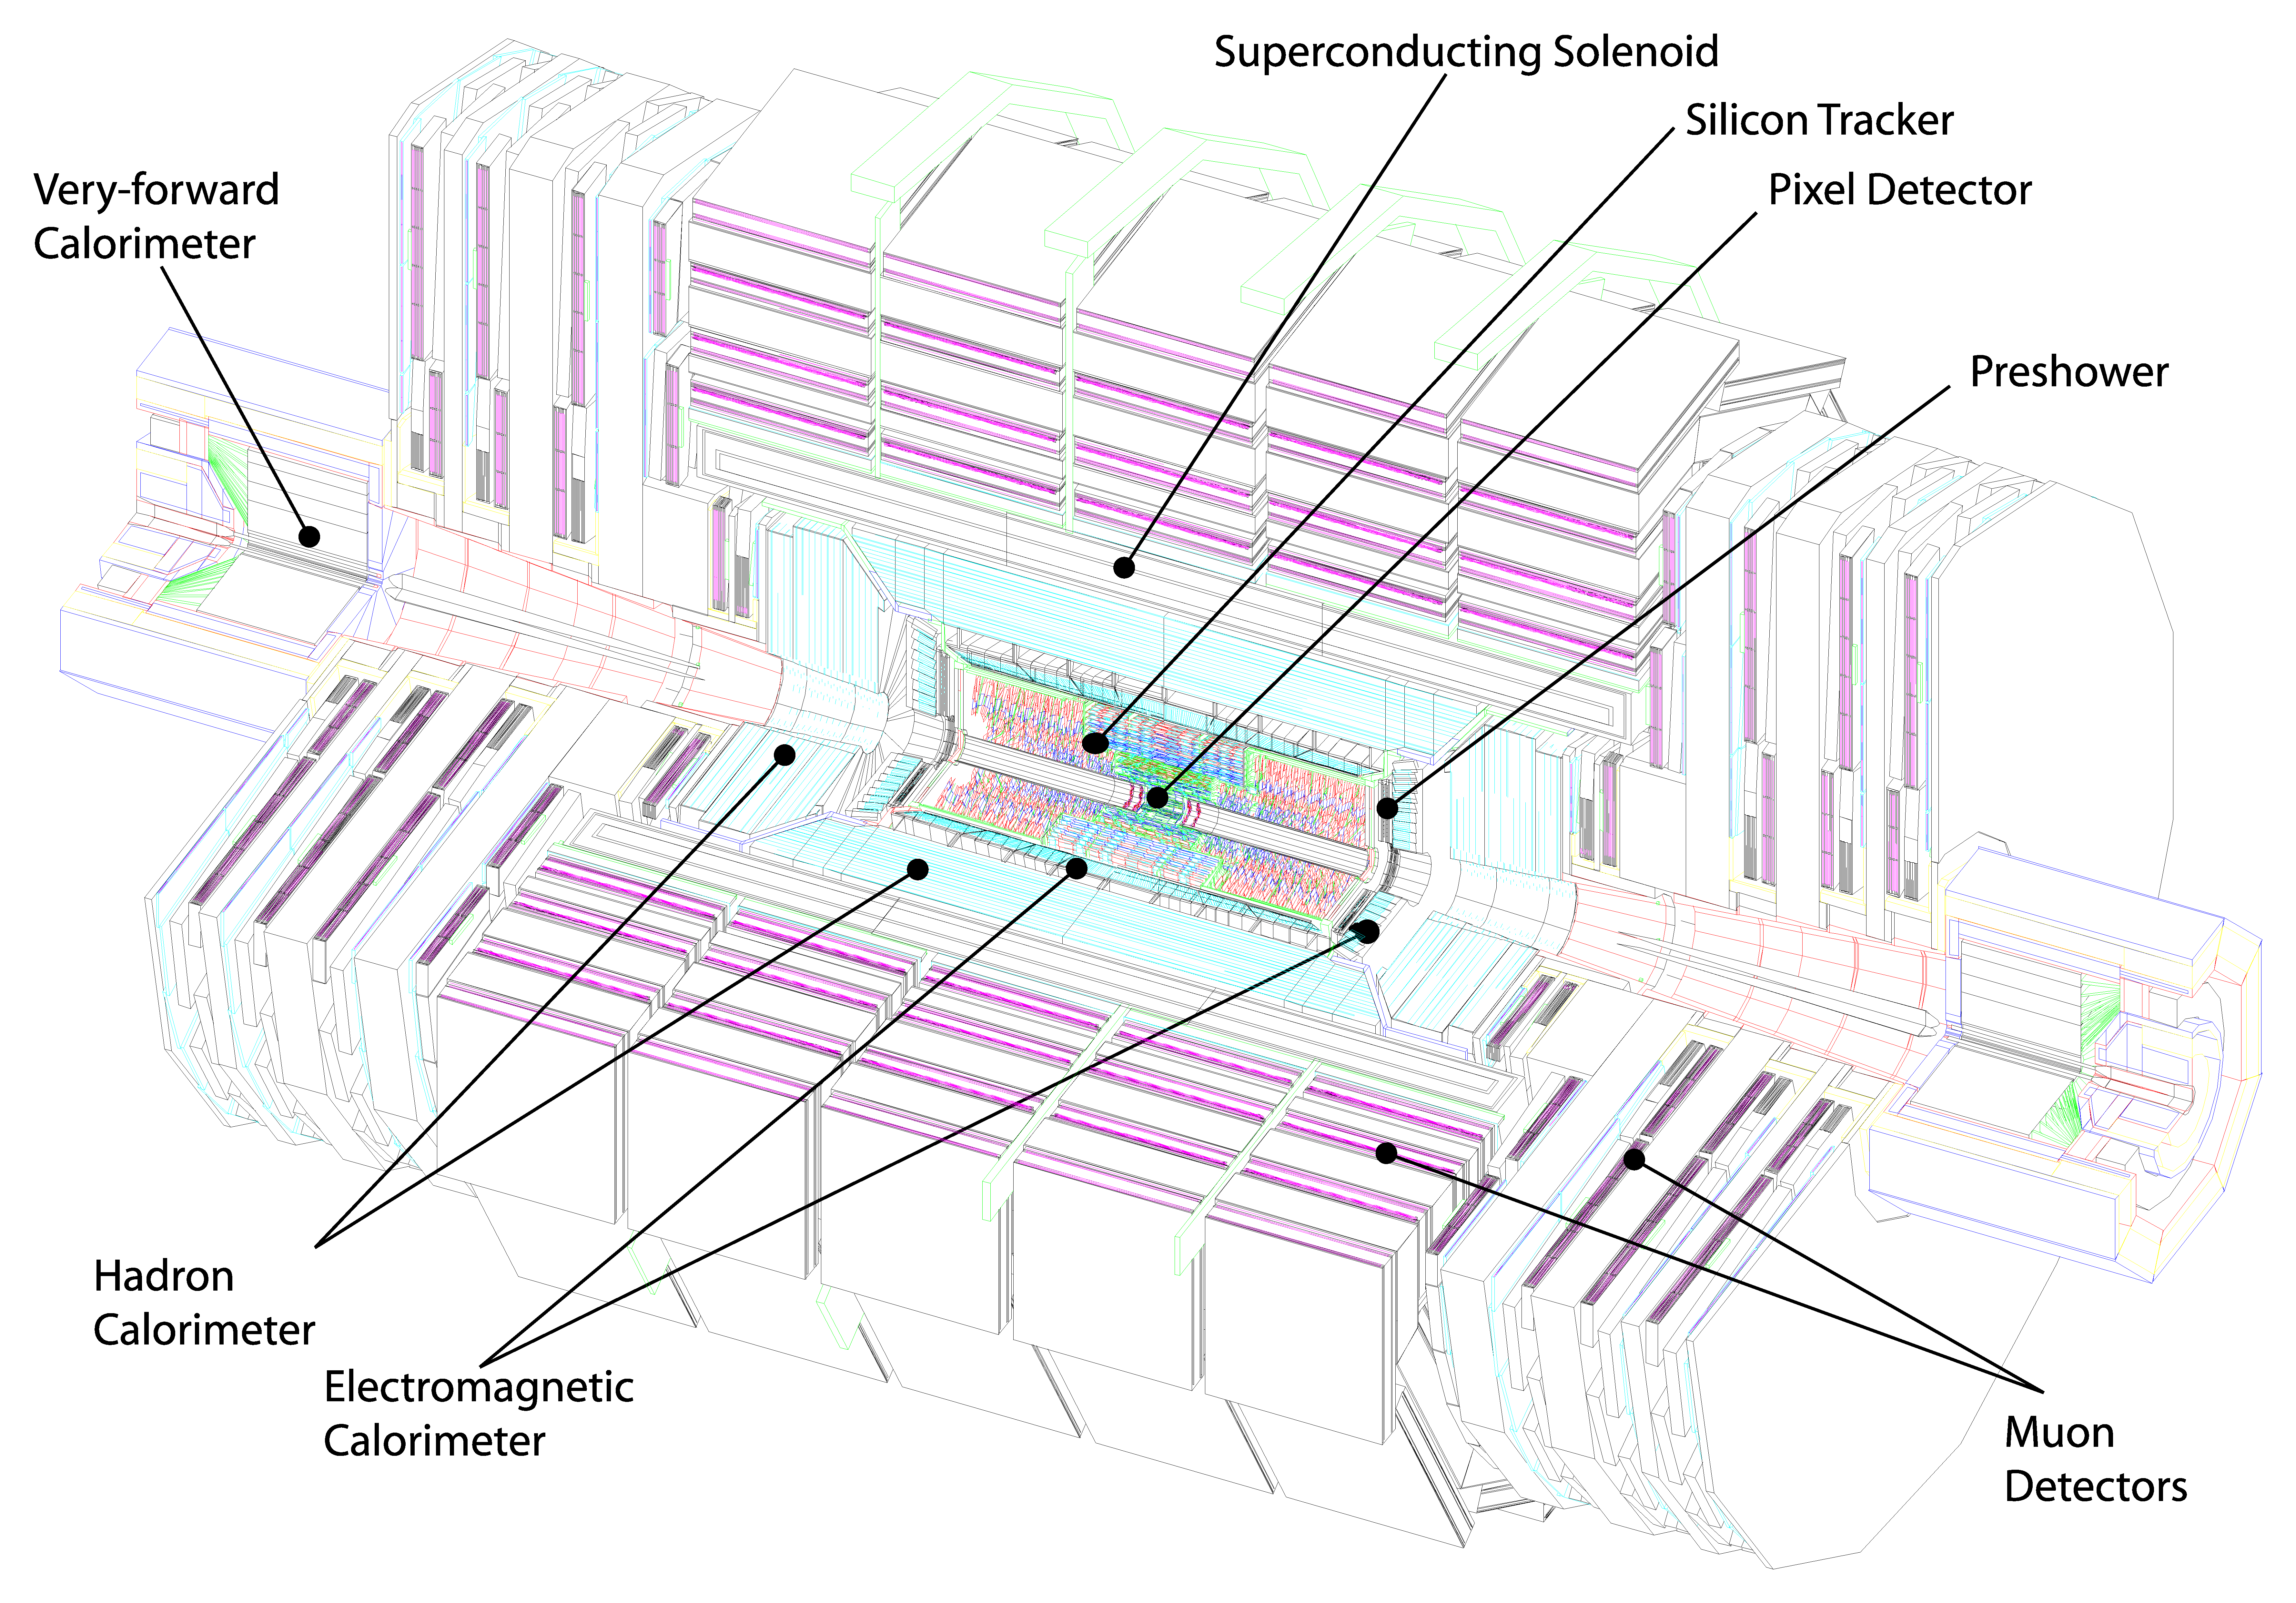
\includegraphics[width=0.7\textwidth]{chapitre2/figs/CMS_2.pdf}
  \caption{Vue en perspective du détecteur CMS}
  \label{fig:cms}
\end{figure}

Les travaux effectués dans cette thèse ayant tous été réalisés à l'aide des données prises par le détecteur CMS, il est intéressant d'étudier plus en détails sa composition.

\bigskip

CMS (figure \ref{fig:cms}) est situé au point 5 du LHC. C'est un détecteur relativement compact, mesurant seulement \SI{28.7}{\m} de long avec un rayon de \SI{7.5}{\m}, pour un poids de \SI{14000}{\tonne}. Afin de pouvoir définir correctement certaines variables, il est nécessaire de définir un repère. L'origine de ce repère ce situe au point d'interaction, et donc au centre du détecteur. L'axe $x$ pointe vers le centre de l'anneau du LHC, et l'axe $z$ est tangent à la direction du faisceau. L'axe $y$, perpendiculaire aux deux autres axes, pointe vers le haut.

L'angle azimutal $\phi \in \left[-\pi, \pi\right]$ est mesuré dans le plan $yx$, à partir de l'axe $x$. L'angle $\theta$, lui, est défini à partir de l'axe $z$ dans le plan transverse $yz$. On préfère cependant utilisé la pseudo-rapidité $\eta$ plutôt que $\theta$, puisque la production de particules est constante suivant $\eta$, mais pas suivant $\theta$. On défini la pseudo-rapidité par
\begin{align*}
  \eta &= -\ln\left[\tan\left(\frac{\theta}{2}\right)\right] = \frac{1}{2} \ln\left(\frac{\abs{\vec{p}} + p_L}{\abs{\vec{p}} - p_L}\right)
\end{align*}

Le LHC étant un collisionneur hadronique, il n'est pas possible de connaître à l'avance l'énergie exacte de la collision. Cependant, le faisceau se déplaçant uniquement le long de l'axe $z$, on sait que le bilan d'énergie dans le plan transverse $xy$ doit être nul. Il est alors commode de définir différente variable \emph{transverse}, tel que l'impulsion transverse ou l'énergie transverse, définis comme la projection vectorielle dans le plan $xy$. On a donc
\begin{align*}
  \pt &= \sqrt{p_x^2 + p_y^2} = \frac{\abs{\vec{p}}}{\cosh\eta} \\
  \et &= E \sin\theta = \frac{E}{\cosh\eta}
\end{align*}

%Pour un détecteur parfait ayant une couverture angulaire totale, on doit avoir $\et = 0$.

L'un des objectifs principaux de CMS, qui figure d'ailleurs dans son nom, est de pouvoir mesurer avec une grande précision l'impulsion des particules, même celles les plus boostées, et particulièrement l'impulsion des muons. On utilise pour cela un puissant champ magnétique de \SI{3.8}{\tesla}, produit grâce à un solénoïde géant, afin de courber la trajectoire des particules. CMS est aussi constitué de couches de de sous-détecteurs, apportant chacun des informations particulières sur la collision, telle que l'énergie des particules, ainsi que leurs trajectoires. Chaque sous-détecteur est décrit en détail dans les sections suivantes.

\begin{figure}[t] \centering
  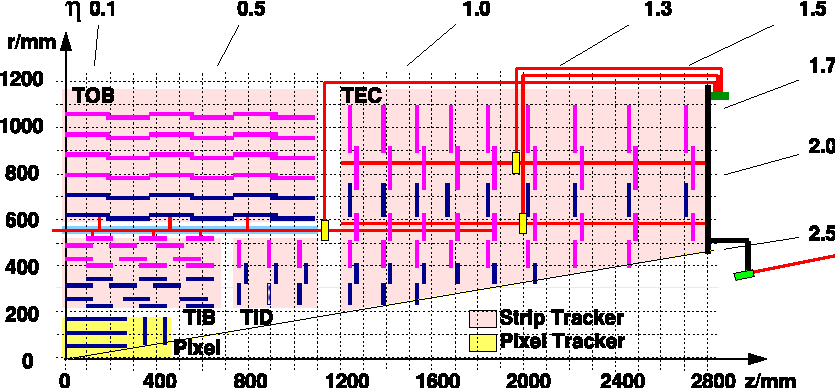
\includegraphics[width=0.7\textwidth]{chapitre2/figs/tracker.pdf}
  \caption{Représentation simplifiée du trajectographe de l'expérience CMS.}
  \label{fig:tracker}
\end{figure}

\subsection{Le trajectographe}

Le trajectographe est l'un des composants les plus important de CMS. Il est en effet chargé de reconstruire la trajectoire courbée des particules chargées, et ainsi d'en déduire leur impulsion. Cylindre d'une longueur de \SI{5.5}{\m} et de \SI{1.1}{\m} de rayon, le trajectographe est composée de deux parties, conçues pour couvrir une région angulaire entre $0 < \eta < \num{2.5}$.

\smallskip

La première partie est le détecteur à pixels. Il est composé de trois couches de détections situées au plus proche du détecteur (à $r = \SI{4}{\cm}$, $r = \SI{7}{\cm}$ et $r = \SI{11}{cm}$), et de quatre disques (bouchons) disposés 2 à 2 à chaque extrémité ($z = \pm \SI{34.5}{\cm}$ et $z = \pm \SI{46.5}{\cm}$). Ce détecteur en silicium comporte environ 65 millions de pixels, mesurant chacun \SI{100}{\um} par \SI{150}{\um}, pour une superficie totale de détection d'environ \SI{1}{\square\m}. Sa résolution est inférieure à $\SI{10}{\um}$ dans le plan $r\phi$ (voir figure \ref{fig:pixel_resolution}) et $\SI{20}{\um}$ en $Z$.

La deuxième partie est le détecteur à micropistes. Englobant le détecteur à pixels, ce détecteur est composé de plus de 10 couches de micropistes en silicium, pour un total d'environ 10 millions de micropistes. On dénombre 4 sous-ensemble :

\begin{description}
  \item[Le TIB] (\emph{Tracker Inner Barrel}) C'est la partie interne du tonneau du trajectographe, composée de 4 couches de micropistes.
  \item[Le TID] (\emph{Tracker Inner enDcaps}) Cette partie complète le TIB et compte trois couches de détection.
  \item[Le TOB] (\emph{Tracker Outer Barrel}) Entourant le TIB, cette partie est constituée de six couches de micropistes.
  \item[Le TEC] (\emph{Tracker EndCaps}) Composée de neuf couches, cette partie complète le TOB.
\end{description}

L'agencement du trajectographe, avec les détecteurs à pixels et à micropistes, est présenté en détails figure \ref{fig:tracker}.

\begin{figure} \centering
  \subcaptionbox{Evolution de la résolution dans le plan $r\phi$ du détecteur à pixel du trajectographe en fonction de la luminosité totale collectée, déterminée à l'aide des données collectées en 2012.\label{fig:pixel_resolution}}[.45\textwidth]{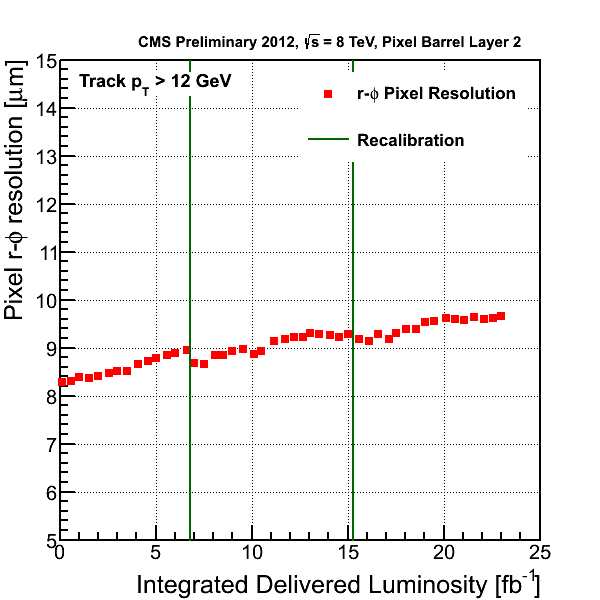
\includegraphics[width=0.45\textwidth]{chapitre2/figs/pixel_detector_resolution_over_time.png}}\hfill
  \subcaptionbox{Efficacité de reconstruction des traces du détecteur à pixel du trajectographe en fonction de la luminosité totale collectée, déterminée à l'aide des données collectées en 2012.\label{fig:pixel_efficiency}}[.45\textwidth]{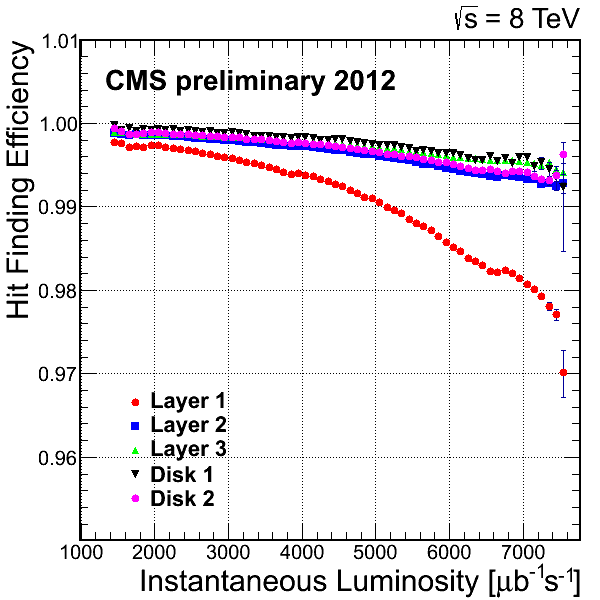
\includegraphics[width=0.45\textwidth]{chapitre2/figs/pixel_detector_efficiency_over_time.png}}
  \caption{Résolution (\subref{fig:pixel_resolution}) et efficacité de reconstruction (\subref{fig:pixel_efficiency}) du détecteur à pixels du trajectographe.}
\end{figure}

\subsection{Le calorimètre électromagnétique}

Situé juste après le trajectographe, le calorimètre électromagnétique (ECAL) sert à mesurer de façon précise l'énergie des électrons et des photons. Sachant qu'un des canaux majeurs d'étude du boson de Higgs est sa désintégration en deux photons, un soin tout particulier a été apportée lors de la conception de ce calorimètre.

Une des contraintes majeures qui a dictée sa conception est l'espace disponible entre le trajectographe et le solénoïde, assez réduit. Ce manque de place a éliminée la technologie la plus avancée à l'époque de la conception, le calorimètre à argon liquide\footnote{C'est la technologie qu'a choisi ATLAS pour son calorimètre électromagnétique.}. Il a au final été choisi d'utiliser un détecteur à scintillation, formé d'un ensemble de cristaux de tungstate de plomb ($PbWO_4$). Le calorimètre couvre une région angulaire entre $0 < \abs{\eta} < 3$, et est séparée en deux parties : le tonneau (EB, pour \emph{ECAL Barrel}, $0 < \abs{\eta} < \num{1.479})$ et le bouchon (EE, pour \emph{ECAL Endcap}, $\num{1.479} < \abs{\eta} < 3$).

\subsubsection{Les cristaux}

Le ECAL est constitué de 76200 cristaux de tungstate de plomb : 61200 dans le tonneau, et 15000 dans les bouchons. Le choix du tungstate de plomb a été dicté par plusieurs contraintes : la résistance aux radiations, le coût, mais principalement un encombrement réduit. En effet, ses cristaux ont été spécialement conçu pour avoir une faible longueur de radiation\footnote{Longueur pour qu'un électron perde $\sfrac{2}{3}$ de son énergie.} ($X_0 = \SI{0.89}{\cm}$), ce qui permet d'utiliser des cristaux ayant une épaisseur modeste ($\num{25.8}X_0$ dans le tonneau, et $\num{24.7}X_0$ dans les bouchons) tout en stoppant les particules même les plus énergétiques. Un autre aspect très intéressant du $PbWO_4$ est son faible rayon de molière (\SI{2.19}{\cm}) \footnote{90\% de l'énergie de la gerbe électromagnétique est contenue dans cylindre rayon le rayon de molière.}. Il est ainsi possible d'utiliser des cristaux ayant des dimensions très réduites (\SI{21.8}{\cm} $\times$ \SI{21.8}{\cm} dans le tonneau, et \SI{24.7}{\cm} $\times$ \SI{24.7}{\cm} dans les bouchons), ce qui permet d'obtenir une très grande granularité en $\eta$ et $\phi$.
En contrepartie de ces excellentes caractéristiques, les cristaux de tungstate de plomb ont un inconvénient majeur : leur réponse est très sensible à la température (\tilde $\SI[per-mode = symbol]{2}{\percent\per\degreeCelsius}$). Il est donc nécessaire de maintenir une température très sable dans ECAL : un système de refroidissement permet de maintenir la température dans le ECAL à $\pm \SI{0.05}{\degreeCelsius}$.

\medskip

Le calorimètre électromagnétique est un détecteur à scintillation : lors du passage d'un électron ou d'un photon, de la lumière est émise en quantité proportionnelle à l'énergie déposée dans le cristal. Afin de collecter cette lumière, des photodétecteurs sont associés à chaque cristal. Les conditions de fonctionnement dans le détecteur étant rude (champ magnétique de \SI{8.3}{\tesla}, très fortes radiations), deux technologies différentes ont été retenues : les photodiodes à avalanches pour le tonneau (APD), et les phototriodes à vide pour les bouchons (VPT).

\subsubsection{Le détecteur à pied de gerbe}

On a vu qu'un des canal de détection les plus prometteur pour le boson de Higgs est sa désintégration en deux photons. Cependant, certains hadrons neutres, tel que le $\pi^0$, peuvent imiter la présence d'un photon énergique lorsqu'ils se désintègrent en deux photons. Ces deux photons sont très proche l'un de l'autre, et la granularité du calorimètre n'est pas suffisante pour les détecter comme deux particules distinctes. A la place, un unique photon énergétique sera détecté. Afin de palier à ce problème, il a été décidé de placer un détecteur à pied de gerbe juste avant le calorimètre électromagnétique, uniquement dans les bouchons\footnote{Un détecteur à pied de gerbe est aussi prévu pour le tonneau, mais n'est pas encore installé}. Ce détecteur, couvrant une région en $\abs{\eta}$ entre \num{1.653} et \num{2.6}, permet d'initier la gerbe électromagnétique avant d'entrer dans le ECAL, grâce à une plaque de plomb et d'aluminium. Composé d'une surface de détection en silicium de \SI{8}{\square\meter}, il possède une granularité bien plus importante que le ECAL, avec des bandes de détection de \SI{2}{\mm} de large. Il est ainsi possible de détecter correctement les photons issus d'un $\pi^0$ boosté.

\begin{figure}[t] \centering
  \subcaptionbox{Réponse relative des cristaux en fonction du temps, pour différentes zones en $\eta$. \label{fig:ecal_transparency}}[0.45\textwidth]{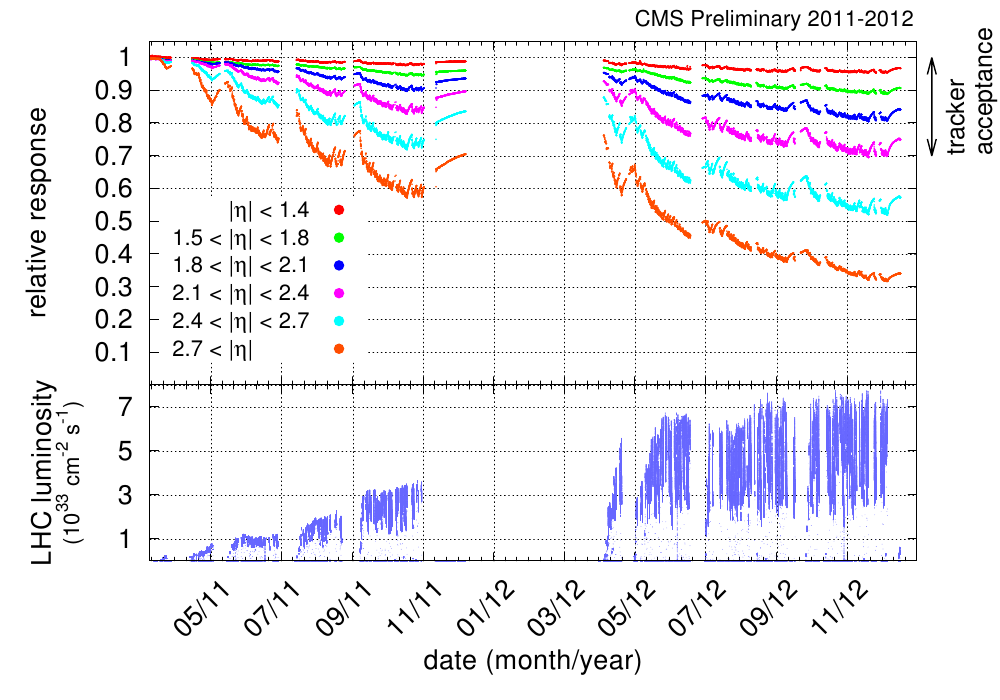
\includegraphics[width=0.45\textwidth]{chapitre2/figs/ecal_transparency.png}} \hfill
  %\subcaptionbox{Résolution relative en énergie des cristaux en fonction de $\eta$ des superclusters.}[0.45\textwidth]{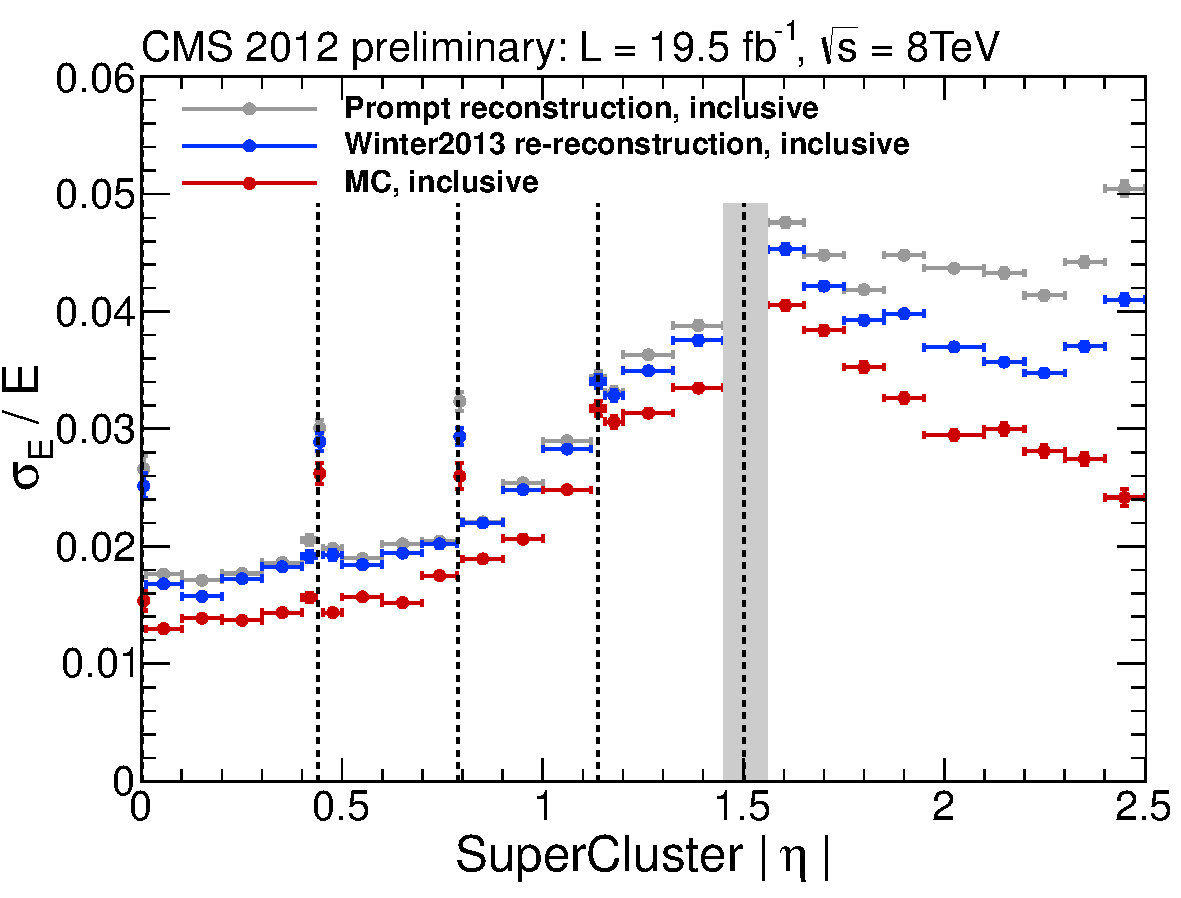
\includegraphics[width=0.45\textwidth]{chapitre2/figs/ecal_resolution.pdf}}
  \subcaptionbox{Effet des corrections de transparence des cristaux sur la masse invariante $M_{ee}$ sur des événements $Z \rightarrow ee$. \label{fig:ecal_corrections}}[0.45\textwidth]{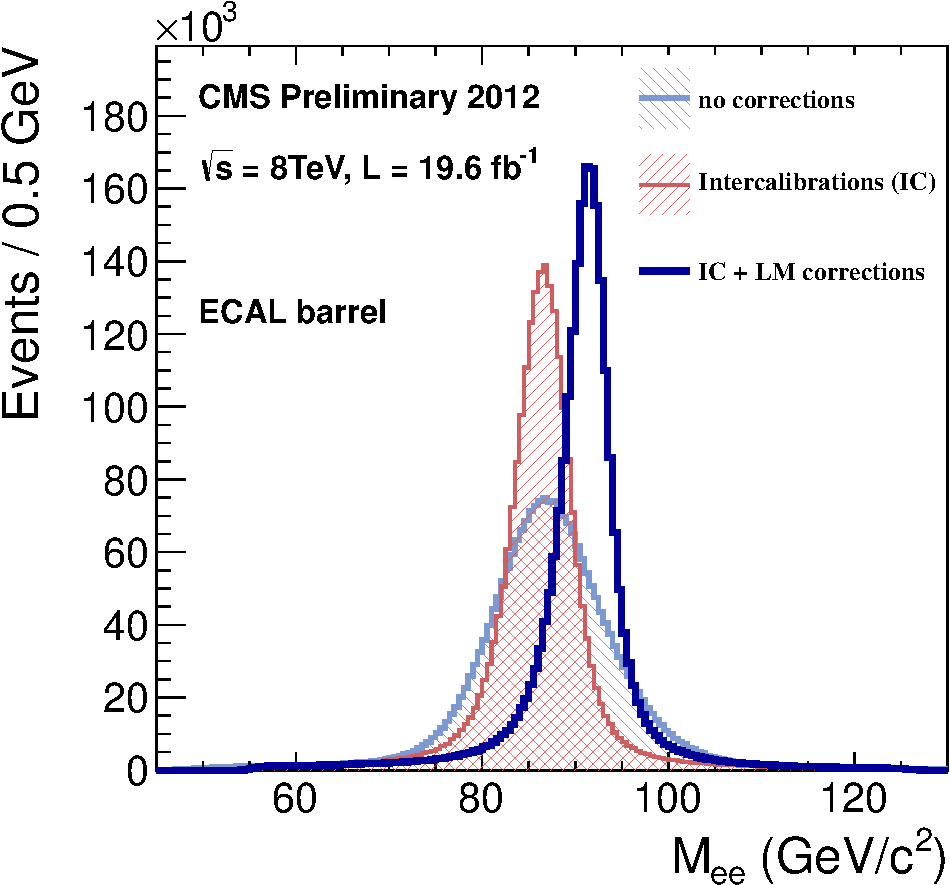
\includegraphics[width=0.45\textwidth]{chapitre2/figs/ecal_corrections_effect.pdf}}
  \caption{Performance des cristaux du ECAL}
  \label{fig:ecal_performance}
\end{figure}

\subsubsection{Performances}

Les cristaux du ECAL sont très sensible aux radiations, et perdent de la transparence au fil du temps. Afin de mesurer cet effet, un système de contrôle a été mis en place. Toutes les 20 minutes, un laser est envoyé dans tous les cristaux enfin de mesurer leur transparence. On peut voir figure \ref{fig:ecal_transparency} la réponse relative des cristaux du ECAL en fonction de la date de prise de données. On voit clairement la diminution de la réponse, du à l'impact des radiations sur les cristaux. Des corrections sont déployées après coup pour corriger cet effet. On peut voir figure \ref{fig:ecal_corrections} l'effet de ces corrections. La courbe hachurée bleue représente le spectre de masse invariante des événements $Z \rightarrow ee$ sans aucune correction. En ajoutant graduellement les corrections de transparence du ECAL, on obtient la courbe rouge, puis la courbe bleue. On voit une très nette amélioration de la valeur moyenne et de la résolution.

\bigskip

La résolution du ECAL peut être paramétrée de la façon suivante :
\begin{align*}
  \left( \frac{\sigma}{E} \right)^2 &= \left( \frac{S}{\sqrt{E}} \right)^2 + \left( \frac{N}{E} \right)^2 + C^2
\end{align*}
où $S$ est le terme stochastique, dû au fluctuation dans l'étalement latéral de la gerbe électronique, $N$ le terme de bruit, dû au bruit des électroniques, et $C$ le terme constant, dû principalement au erreurs d'intercalibrations.

Elle a été évaluée lors de tests sur faisceaux en 2006 à
\begin{align*}
  \left( \frac{\sigma}{E} \right)^2 &= \left( \frac{\SI{2.8}{\%}}{\sqrt{E}} \right)^2 + \left( \frac{\num{0.12}}{E} \right)^2 + \left(\SI{0.30}{\%}\right)^2
\end{align*}
ce qui équivaut, pour un électron de $E = \SI{120}{\GeV}$, à $\sigma = \SI{1.90}{\GeV}$. Récemment, la résolution du ECAL a été évaluée en utilisant les données collectées en 2012. On peut voir figure \ref{fig:ecal_resolution} l'évolution de la résolution en fonction de la position angulaire des superclusters. On constate que pour $\abs{\eta} < 1.3$, la résolution est inférieure à \SI{3}{\%}, soit $\sigma = \SI{3.6}{\GeV}$. C'est donc une excellente performance pour le détecteur.

\begin{figure} \centering
  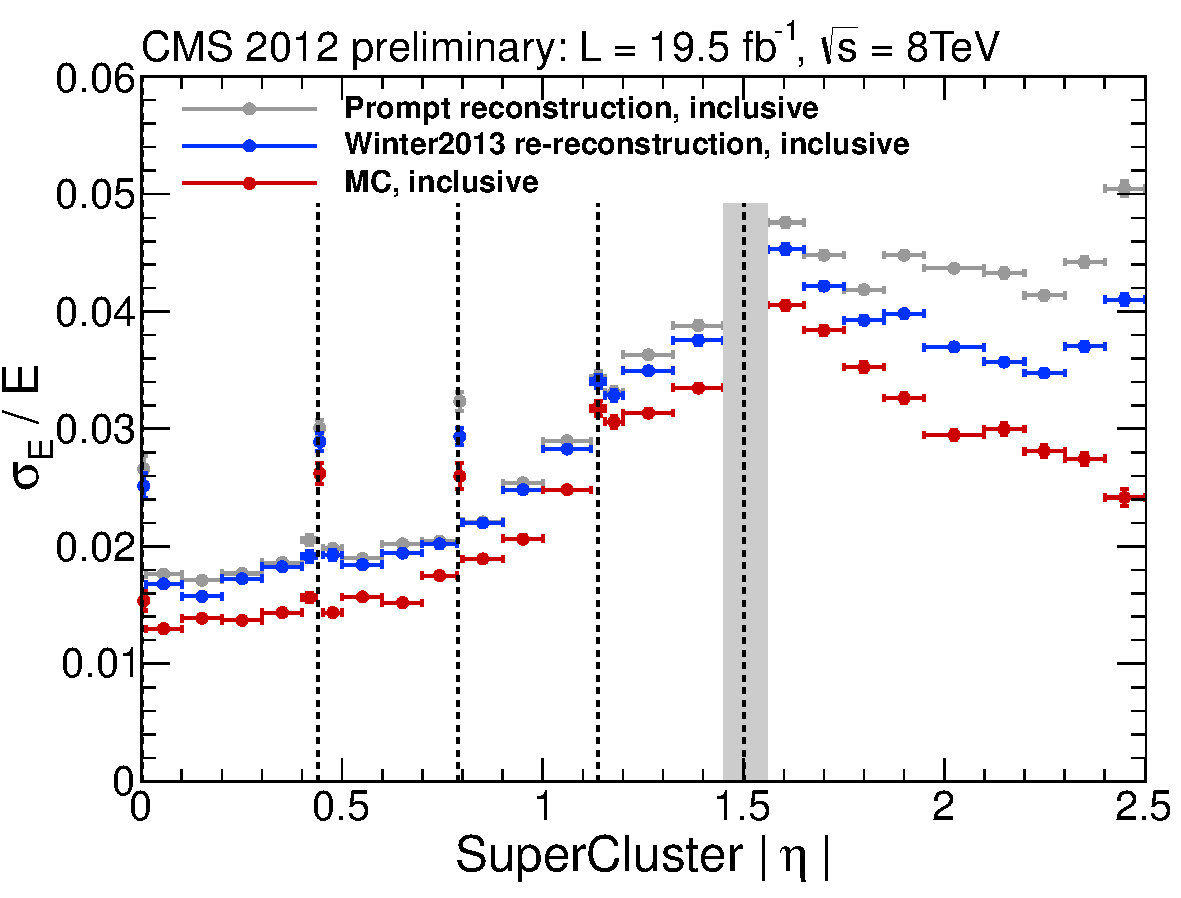
\includegraphics[width=0.4\textwidth]{chapitre2/figs/ecal_resolution.pdf}
  \caption{Évolution de la résolution totale du ECAL en fonction de la position angulaire $\eta$ du supercluster}
  \label{fig:ecal_resolution}
\end{figure}

\subsection{Le calorimètre hadronique} \label{sec:hcal}

Le rôle du calorimètre hadronique (HCAL, pour \emph{Hadronic CALorimeter}) est de mesurer l'énergie des hadrons neutres et chargés, grâce à l'utilisation d'un détecteur à échantillonnages. Une succession de couches d'absorbant et de scintillateurs permettent de déterminer la trajectoire et l'énergie d'une particule incidente. De façon analogue au calorimètre électromagnétique, il est constitué de deux parties : une partie tonneau et deux bouchons.

L'absorbant retenu pour le tonneau et les bouchons est le laiton. Étant installé au sein d'un puissant champ magnétique, il fallait en effet choisir un métal para-magnétique. Le laiton a aussi l'avantage d'être quasi transparent pour les muons : leur détection intervenant après le HCAL, il est en effet important que les muons ne perdent pas d'énergie dans le HCAL, au risque de biaiser l'estimation de leur impulsions. Chaque couche d'absorbant mesure \SI{5}{\cm} d'épaisseur dans le tonneau, et \SI{8}{\cm} dans les bouchons. Entre chaque couche d'absorbant se trouve une couche de scintillateur plastique de \SI{3.7}{\mm} d'épaisseur. La lumière produite lors du passage d'une particule est collectée par des fibres optiques, puis amplifiée par des photodiodes hybrides.

\medskip

Le tonneau couvre une zone angulaire entre $0 \leq \abs{\eta} < \num{1.48}$, et est composé de deux parties différentes. La première partie, le HB, mesure \SI{89}{\cm} de profondeur, soit seulement \SI{5.82}{\lambda_0}\footnote{La longueur d'interaction nucléaire, $\lambda_0$, est une longueur caractéristique des matériaux. C'est la longueur après laquelle \SI{36.8}{\%} ($\sfrac{1}{e}$) des hadrons sont absorbés par le milieu. le laiton, on a $\lambda_0 = \SI{16.42}{\cm}$}. Cette longueur est insuffisante pour absorber la totalité de la gerbe hadronique. Une deuxième partie, le HO, à donc été ajouté, située à l'extérieur du solénoïde. L'aimant sert alors d'absorbeur, et le HO détecte les gerbes longues ou tardives. Les bouchons couvrent eux une zone angulaire entre $1.48 \leq \abs{\eta} < \num{3}$. La longueur totale du calorimètre est, en incluant le ECAL, d'environ \SI{10}{\lambda_0}, suffisant pour stopper la gerbe hadronique.

\bigskip

Ainsi constitué, le HCAL couvre une région angulaire entre $0 \leq \abs{\eta} < \num{3}$. Cependant, afin de correctement mesurer l'énergie manquante dans la collision, il est important de couvrir au maximum tout l'espace angulaire. Ainsi, un détecteur parfait couvrirait une zone $0 \leq \abs{\eta} < \infty$. Ce n'est malheureusement pas possible puisqu'il faut laisser un espace libre pour le faisceau de particules. Le HCAL comprend une troisième partie, plus à l'avant, couvrant une zone angulaire entre $\num{3} \leq \abs{\eta} < \num{5}$, le HF. C'est un cylindre de \SI{130}{\cm} de rayon, situé à \SI{11.2}{\m} du point d'interaction. D'une longueur de \SI{165}{\cm} (\tilde \SI{10}{\lambda_0}), il est constitué d'un absorbeur en acier, dans lequel sont introduites des fibres optiques en quartz. Les particules chargées entrant dans le milieu émettent de la lumière Cherenkov, collectée par les fibres puis amplifiée. Ce détecteur est ainsi principalement sensible à la partie électromagnétique des gerbes hadroniques.

\fxerror{Parler de la résolution ?}

\fxerror{Mettre quelques lignes sur la mesure de la luminosité dans le HF}

\subsection{Le solénoïde}

L'aimant supraconducteur de CMS a été conçu afin de fournir un champ magnétique de \SI{3.8}{\tesla}. De forme cylindrique de rayon \SI{6}{\m}, il est long de \SI{12.5}{\meter}, il est parcouru par un courant électrique de \SI{19.14}{\kilo\ampere}. Afin de maintenir son état supraconducteur, l'aimant est refroidi par un système de cryostat fonctionnant à l'hélium superfluide. Il est ainsi constamment maintenu à une température de \SI{1.9}{\kelvin}.

On a vu déjà précédemment l'intérêt d'un puissant champ magnétique. En effet, la trajectoire d'une particule chargée se courbe en présence d'un champ magnétique, avec un rayon de courbure proportionnel à son impulsion :
\begin{align*}
  r &= \frac{p}{qB}
\end{align*}
avec $r$ le rayon de courbure de la trajectoire, $p$ l'impulsion, $q$ la charge de particule et $B$ l'intensité du champ magnétique. Plus $r$ est petit, plus il est simple à mesurer, puisque la courbure de la trajectoire sera plus prononcée. Afin de mesurer de façon précise l'impulsion des particules, même les plus boostées, il est donc nécessaire d'utiliser un champ magnétique puissant afin de minimiser $r$.

\subsection{Le détecteur à muons}

\begin{figure}[tb] \centering
  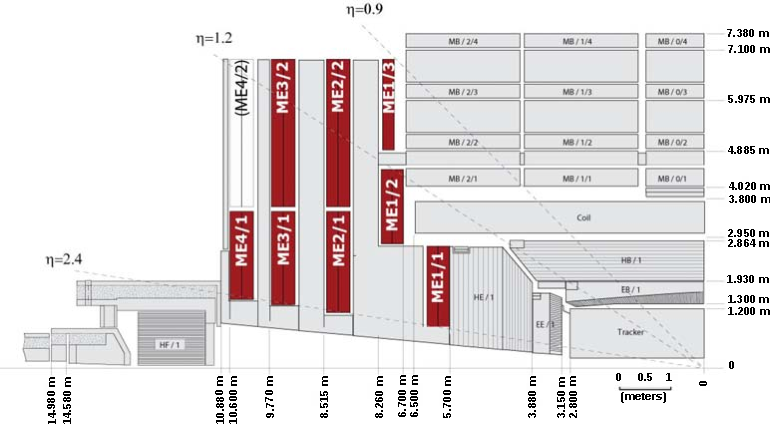
\includegraphics[width=0.8\textwidth]{chapitre2/figs/CSC.pdf}
  \caption{Vue un-quart du détecteur CMS. Les chambres à pistes cathodiques des bouchons sont illustrées en rouge.}
  \label{fig:cms_csc}
\end{figure}


Le détecteur à muons joue un rôle central dans CMS, puisqu'il couvre trois fonctions principales : identifier les muons, mesurer leur impulsion, et assurer une partie du déclenchement. C'est la partie la plus externe de CMS, que seul les muons peuvent atteindre. Il est ainsi beaucoup plus facile de mesurer l'impulsion de ces particules, grâce à l'éloignement entre le trajectographe et ce détecteur.

\begin{figure}[p] \centering
  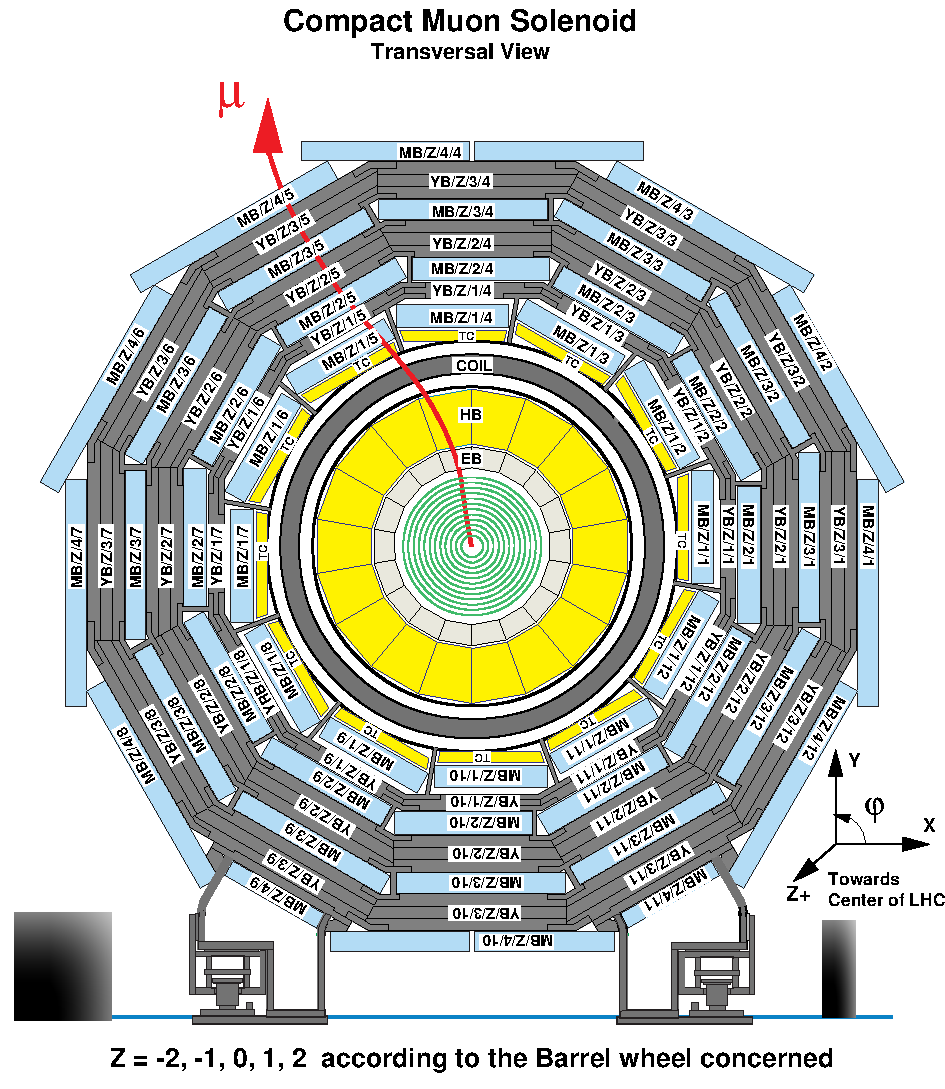
\includegraphics[width=0.95\textwidth]{chapitre2/figs/CMS_transverse_view.pdf}
  \caption{Agencement des tubes à dérives dans le tonneau de CMS (vue transverse). Chaque rectangle bleue correspond à un tube à dérive.}
  \label{fig:cms_dt}
\end{figure}

On trouve trois différentes technologies au sein du détecteur à muons : les tubes à dérive (DT, pour \emph{Drift Tube}) et les chambres à pistes cathodique (CSC, pour \emph{Cathod Strip Chamber}), utilisé pour les mesures liées aux muons, et les détecteurs à plaques résistives (RPC, pour \emph{Resistive Plate Chamber}) utilisés par le système de déclenchement.

\begin{description}
  \item[Les tubes à dérives] Installés dans le tonneau (voir figure \ref{fig:cms_dt}), ces détecteurs couvrent une zone angulaire $\abs{\eta} < 1.2$. On en compte 250 dans le détecteur.
  \item[Les chambres à pistes cathodiques] Ces détecteurs sont utilisés dans les bouchons (voir figure \ref{fig:cms_csc}), là où le champ magnétique n'est pas constant et le taux de radiation élevé. 540 de ces modules sont installés, couvrant une zone angulaire $\num{0.9} < \abs{\eta} < \num{2.4}$.
  \item[Les détecteurs à plaques résistives] Présent à la fois dans le tonneau et dans les bouchons, ils permettent d'assurer une partie du déclenchement. En effet, leur temps de réponse est bien inférieur à \SI{25}{\ns}, ce qui permet de décider très rapidement si un événement est digne d’intérêt ou s'il peut être jeté.
\end{description}

%\subsubsection{Performances}

\subsection{Le système de déclenchement}

\begin{figure} \centering
  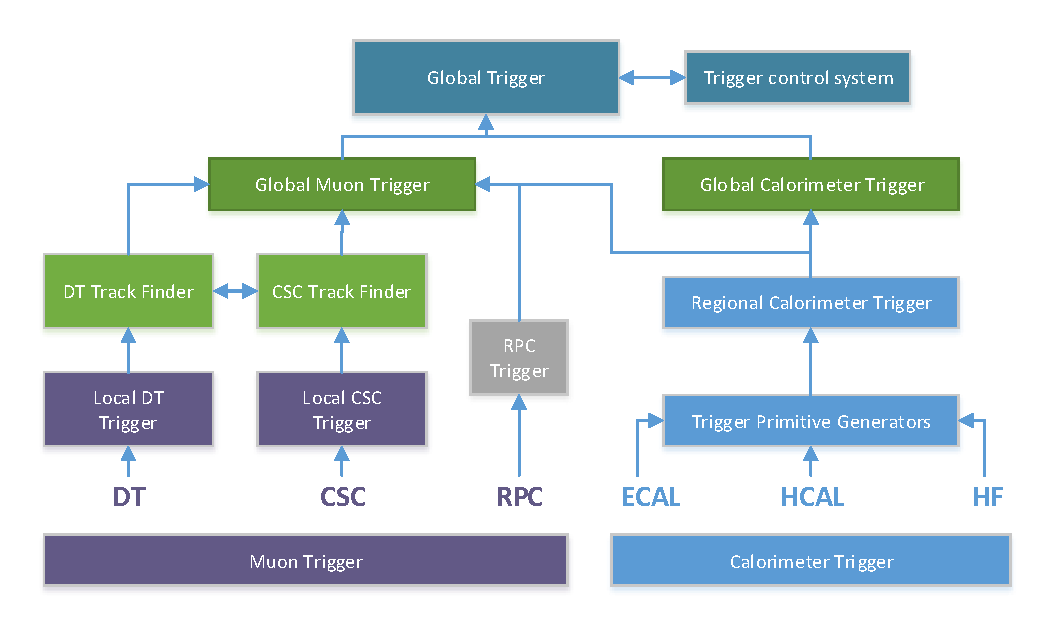
\includegraphics[width=0.7\textwidth]{chapitre2/figs/L1.pdf}
  \caption{L'architecture du déclencheur de niveau 1}
  \label{fig:l1}
\end{figure}

Aux conditions nominales, le temps entre chaque collision est de \SI{25}{\ns}, soit une fréquence de \SI{40}{\mega\hertz}. En estimant la taille d'un événement à environ \SI{1}{\mega\octet}, on obtient alors un débit de données de \SI{40}{\tera\octet\per\second}, débit qu'aucun système de stockage n'arrive à atteindre. Il est donc nécessaire de réduire ce débit en jetant des événements. Tout l'enjeu est de réussir à jeter des événements dont on sait à l'avance qui ne seront pas intéressant (pas de collision de grande intensité, bruit trop important, \ldots). On utilise pour cela un système de déclenchement (\emph{trigger}), composé dans CMS de deux niveaux : le niveau 1 (L1, figure \ref{fig:l1}) et le HLT (\emph{High Level Trigger}, pour déclencheur de haut niveau, figure \ref{fig:daq}). Ces systèmes doivent être capable de décider de garder ou non un événement en temps réel.

\begin{description}
  \item[Le L1] Ce premier niveau de déclenchement réduit le taux d’événements à \SI{100}{\kHz}, à l'aide d'un système électronique ultra-rapide. En utilisant directement les informations provenant du détecteur à muons et des calorimètres, la décision de garder ou non l'événement est prise en moins de \SI{3.2}{\us}. Cette électronique est hautement configurable, et peut être reconfigurée à tout moment. Ainsi, 128 algorithmes de déclenchement tournent en parallèle, ce qui permet de fournir un lot de données adaptées aux besoins des analyses de physique.
  \item[Le HLT] Le taux d'événements en sortie du L1 est encore trop important, et doit être réduit à environ \SI{100}{\Hz} afin d'être stockable en temps réel. Le HLT est chargée d'effectuée cette sélection. Pour cela, une ferme d'ordinateurs est installée à proximité du détecteur et sélectionne les événements digne d’intérêt. Il dispose des données de tous les sous-détecteurs et effectue une reconstruction rapide afin d'obtenir une description de l'événement en terme d'objets physiques plutôt qu'en terme de signaux électriques. Le temps moyen alloué au HLT pour prendre une décision est d'environ \SI{50}{\ms}.
\end{description}

\begin{figure}[tb] \centering
  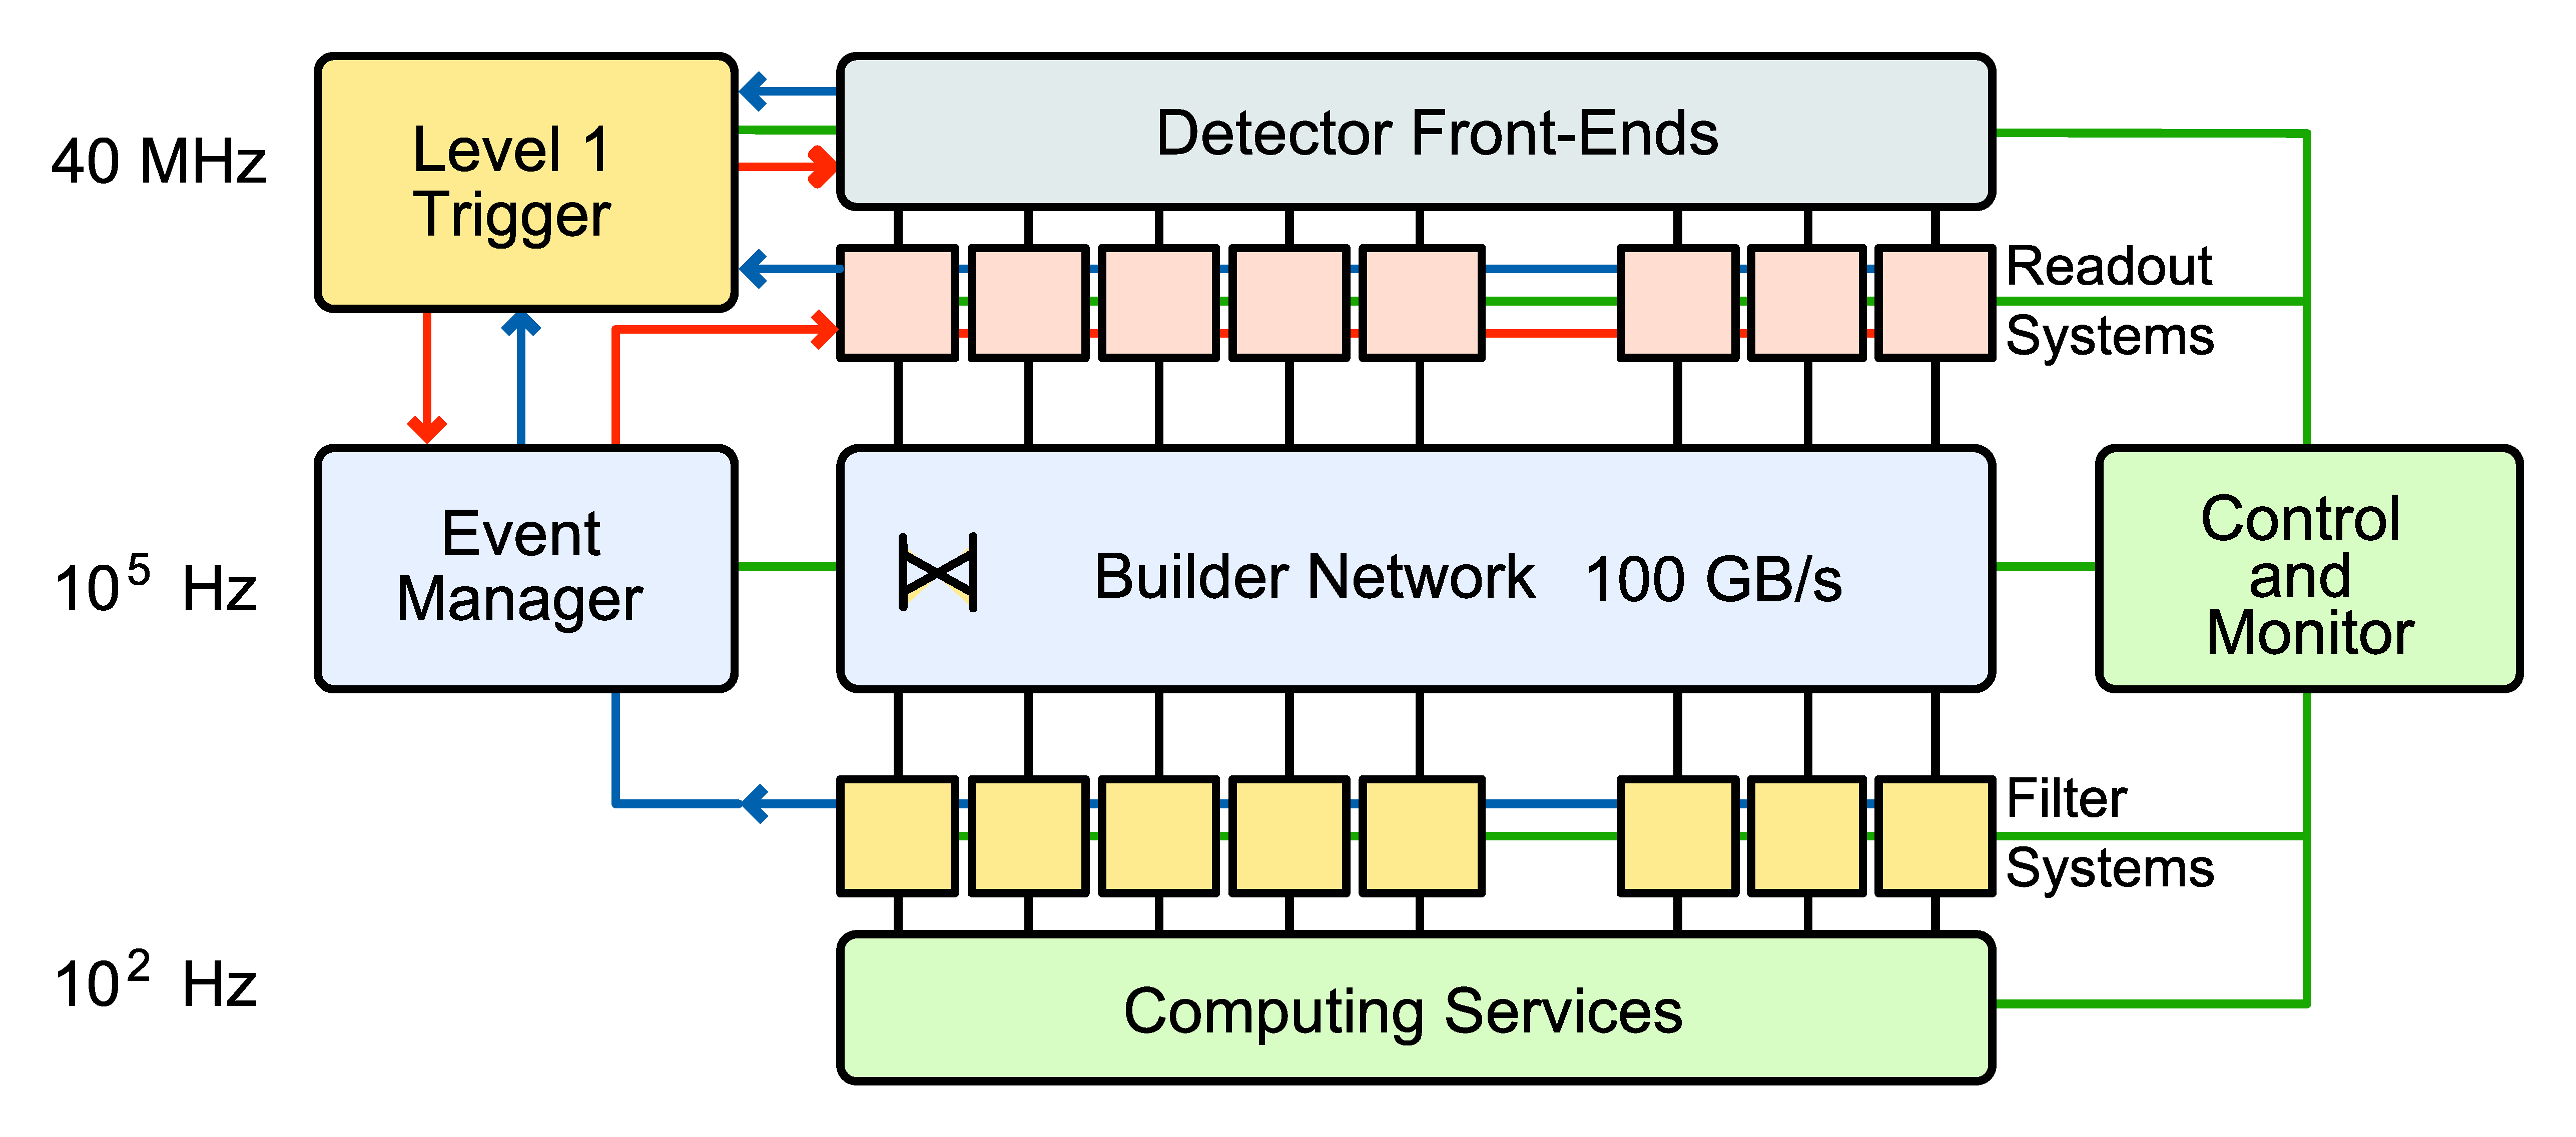
\includegraphics[width=0.7\textwidth]{chapitre2/figs/DAQ.pdf}
  \caption{Schéma de la chaîne d'acquisition de données de CMS}
  \label{fig:daq}
\end{figure}

Une fois accepté, l'événement est stocké de façon définitive dans un centre de stockage à haute redondance, le \emph{Tier-0}.

\section{Conclusion}

Tout au long de ce chapitre, on a vu comment le LHC, et le détecteur CMS, ont été pensé afin d'enrichir nos connaissances sur la physique du Modèle Standard. De nouvelles perspectives s'ouvrent dans le recherche de nouvelles physique au delà du Modèle Standard. Mais pour que les analyses de physique puisse travailler, il faut dans un premier temps reconstruire les collisions, c'est-à-dire convertir les signaux électriques issus des sous-détecteurs en objet physique (électrons, muons, \dots). Les méthodes employées par CMS sont décrites en détails dans le chapitre suivant.